\documentclass[11pt, oneside]{article}   	% use "amsart" instead of "article" for AMSLaTeX format
\usepackage{geometry}                		% See geometry.pdf to learn the layout options. There are lots.
\geometry{letterpaper}                   		% ... or a4paper or a5paper or ... 
%\geometry{landscape}                		% Activate for for rotated page geometry
%\usepackage[parfill]{parskip}    		% Activate to begin paragraphs with an empty line rather than an indent
\usepackage{graphicx}				% Use pdf, png, jpg, or eps� with pdflatex; use eps in DVI mode
								% TeX will automatically convert eps --> pdf in pdflatex		
\usepackage{amssymb}
\usepackage{amsmath}

\title{Notes on Reconfiguration Among Clutter}
%\date{}							% Activate to display a given date or no date

\begin{document}
\maketitle

\section*{Introduction}
In these notes we examine the problem of grasping an object in a cluttered environment.  We categorize the clutter into two groups: static and movable objects. We allow the robot to push any movable object in order to clear a path for grasping the target object.  The robot must avoid contact with static obstacles.  

\section*{Related Work}


\section*{Problem Formulation}
We now provide a more formal description of the problem and introduce notation used throughout the remainder of these notes. As stated previously, we wish to solve the problem of grasping an object, $G$, in a cluttered environment.  Specifically, we say that we have a robot operating in an environment with both static and movable objects.  Let $O = \{O_1, ..., O_k\}$ be the set of static objects.  These objects should be treated as obstacles. Contact between the robot and these objects is forbidden.  Let $M = \{M_1,...,M_n\}$ be a set of movable objects.  These objects can be displaced via contact with the robot. We require that this displacement does not introduce contact between any two objects in $M$ nor does it introduce contact between an object in $M$ and an object in $O$.  Finally, we cannot introduce contact between any object in $M$ and our goal object $G$.  We treat our goal object as a movable object and identify the same contact constraints as any object in $M$, but identify it separately.  We say that a movable object can be displaced when the robot is touching the object.

Let $C_R$ identify the configuration space of the robot.  Let $G_R$ identify the configuration space of the target object, $G$. We can define our goal as a set of configurations, $Q_G = \{q_t \in C_R | f(q_t, g_t) = 0 \}$, where $f(q_t, g_t) = 0$ when our goal object in pose $g_t$ can be stably grasped by the robot in configuration $q_t$.  Let $C_{M_i}$ represent the configuration space of $M_i$.  We can then formalize our problem as follows: given an initial configuration of the robot, $q_0 \in C_R$, an initial configuration of the target object, $g_0 \in G_R$ and an initial configuration for each movable objects, $(c^{M_1}_0,...,c^{M_n}_0) \in (C_{M_1},...,C_{M_n})$, we want to find a path from $q_0$ to any configuration $q_t \in Q_G$ that is collision-free.  

\subsection*{Events}
Here we define the concept of a "contact event."  We define a set of contact indicators, $(I^{M_1},...,I^{M_n}) \in \{0,1\}$ where $I^{M_i} = 1$ if the robot is in contact with movable object $M_i$ and $0$ otherwise.  We can then say a contact event is one where $I^{M_i}_{t-1} \neq I^{M_i}_{t}$ for any $i$.  Informally, we define such an event as any moment in which the contact state between the robot and a movable object changes.  

\subsection*{Actions}
Ultimately we wish to produce a path defined by a sequence of actions, $a_0,...,a_m$ such that when applied to the state $q_0$ the resulting state is a state $q_m \in Q_G$.  We can parameterize these actions as follows:
\[a_t = \left[ \dot{v}, \dot{\theta}, \dot{a}, \Delta t \right] \]
where $\dot{v}$ is the forward velocity of the manipulator, $\dot{\theta}$ is the rotational velocity of the manipulator, $\dot{a}$ is the aperture of the end-effector and $\Delta t$ is the duration of the action.

\begin{figure}[h]
\centering
\label{fig:action_events}
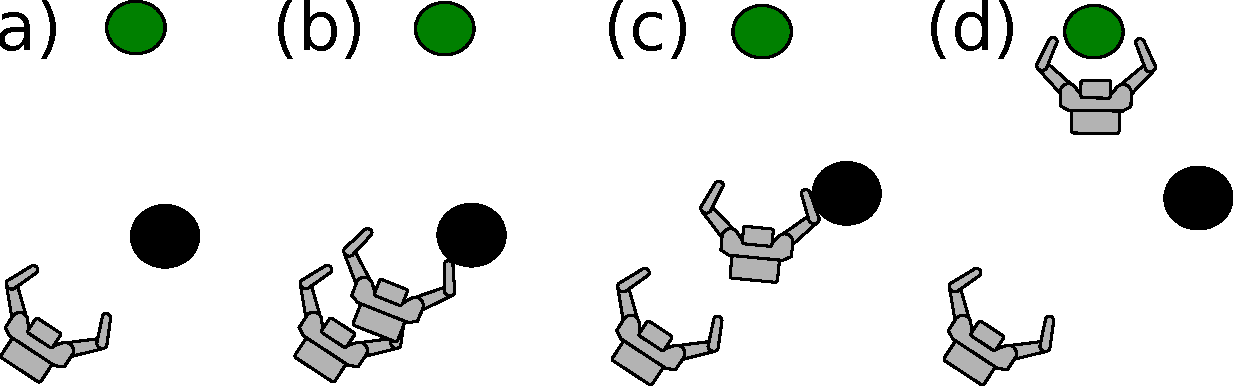
\includegraphics[width=0.8\textwidth]{action_events}
\end{figure}
We note that an action can encompass multiple events.  Consider the action depicted in Figure ~\ref{fig:action_events}.  During execution of this action, the robot starts out of contact with any movable obstacle.  The robot then makes contact with obstacle $M_2$, triggering a contact event (Figure ~\ref{fig:action_events}).  After pushing the obstacle out of the way the robot loses contact with the obstacle, triggering a second contact event (~\ref{fig:action_events}).  Thus we can say we have a one-to-many relationship between actions and events.  This will be important during formulation of our algorithm.

\section*{Building a Tree}

\end{document}
